\section{Netzwerk}
\begin{frame}{Ethernet}{�ber USB}
 \begin{itemize}
  \item Der Befehl \cod{ifconfig}
  \begin{itemize}
   \item \cod{ifconfig} f�r den �berblick
   \begin{itemize}
    \item auf dem \target 
	\item auf dem \host
   \end{itemize}
   \item \cod{ifconfig {\em ifc} {\em ip} up} auf dem \host
   \begin{description}
    \item[ifc] das Interface, die (virtuelle) Netzwerkkarte
	\item[ip] Internetadresse vom \host
	
	typisch: 
	\begin{itemize}
	 \item Netzwerk \cod{192.168.7.*}
	 \item Rechner im Netzwerk \cod{192.168.7.\bf X}
	\end{itemize}
   \end{description}
  \end{itemize}
 \end{itemize}
\end{frame}

\begin{frame}{Die Tools}{f�r die Verbindung}
\begin{block}{Wichtig}
 \begin{itemize}
  \item \cod{ifconfig} f�r die Netzschnittstelle
  \item \cod{ping} f�r den Verbindungstest
  \item \cod{ssh} f�r die Verbindung
 \end{itemize}
 \end{block}
 \see{net-setup.txt}
 \begin{block}{Weiterf�hrend}
 \begin{itemize}
  \item \cod{nmap} f�r Portscans
  \item Ein DHCP Server z.B. \cod{dnsmasq}
  \item \cod{wireshark} f�r die Netz�berwachung
 \end{itemize}
 \end{block}
\end{frame}


\subsection{ssh}
\begin{frame}{SSH}{Secure Shell}
 \begin{description}
  \item[shell] \cod{ssh name@ip} 
  \begin{description}
   \item[name] Benutzername auf dem \target
   \item[ip] Internetadresse vom \target 
  \end{description}
  \item[mount] \cod{sshfs name@ip:directory mount-point}
  \begin{description}
   \item[directory] auf dem \target
   \item[mount-point] auf dem \host
  \end{description}
 \end{description}
\end{frame}

\begin{frame}{ssh}{Secure Shell}
 \begin{description}
  \item[command] \cod{ssh {\em name@ip}} 
  \begin{description}
   \item[name] Benutzername auf dem \target
   \item[ip] Internetadresse vom \target 
  \end{description}
 \end{description}
\end{frame}

\begin{frame}{sshfs}{mount}
 \begin{description}
  \item[command] \cod{sshfs name@ip:directory mount-point}
  \begin{description}
   \item[directory] auf dem \target
   \item[mount-point] auf dem \host
  \end{description}
 \end{description}
 \begin{center}
  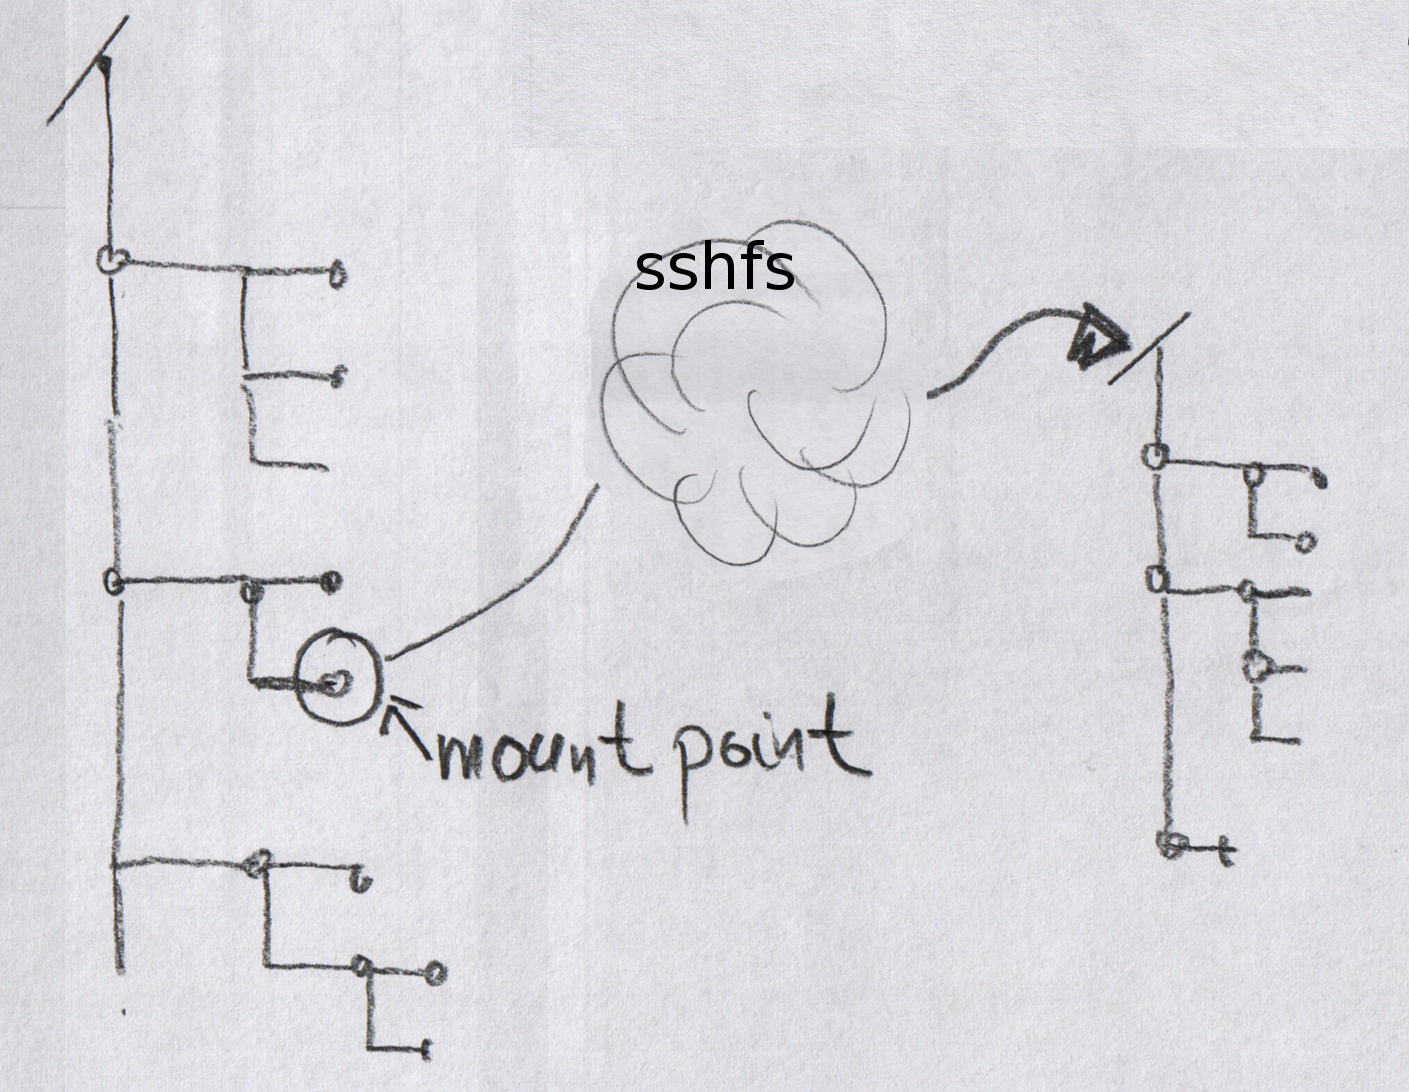
\includegraphics[height=4cm]{sshfs.png}
 \end{center}
\end{frame}

\begin{frame}{Konfiguration \cod{SSH}}{Server}
 \begin{itemize}
  \item \cod{ssh-keygen -t{\em type} -f /etc/ssh/ssh\_host\_{\em type}\_key}
  \begin{itemize}
   \item mit \cod{{\em type}=rsa\textbar dsa}
  \end{itemize}
  \item \cod{ssh-copy-id}
  \remark{Auf dem {\em Target}}
 \end{itemize}
 
\end{frame}
